\documentclass[a4paper]{article}
\usepackage[utf8]{inputenc}
\usepackage{textcomp}
\usepackage{geometry}
\geometry{ left=2cm, right=2cm, top=2cm, bottom=2cm, bindingoffset=5mm}
\usepackage{graphicx}
\usepackage{xcolor}
\usepackage{hyperref}
\date{}
\author{}
\usepackage{fancyhdr}
\pagestyle{fancy}
\fancyhf{}
\fancyhead[R]{2973140 - Felix Bühler \\ 2892258 - Gerhard Breul \\  3141241 - Jamie Ullerich}
\fancyhead[L]{Information Visualisation and Visual Analytics \\ WS 2019/20 }
\renewcommand{\headrulewidth}{0.5pt}
\usepackage{tikz}
\usetikzlibrary{calc}
\usepackage{amsmath}
\usepackage{cleveref}
\usepackage{subcaption}

\usepackage{changepage,lipsum,titlesec}
\titleformat{\section}[block]{\bfseries}{\thesection.}{1em}{}
\titleformat{\subsection}[block]{}{\thesubsection}{1em}{}
\titleformat{\subsubsection}[block]{}{\thesubsubsection}{1em}{}
\titlespacing*{\subsection} {2em}{3.25ex plus 1ex minus .2ex}{1.5ex plus .2ex}
\titlespacing*{\subsubsection} {3em}{3.25ex plus 1ex minus .2ex}{1.5ex plus .2ex}


\title{\textbf{Assignment 8}}

\begin{document}
\maketitle 
\thispagestyle{fancy}


\fbox{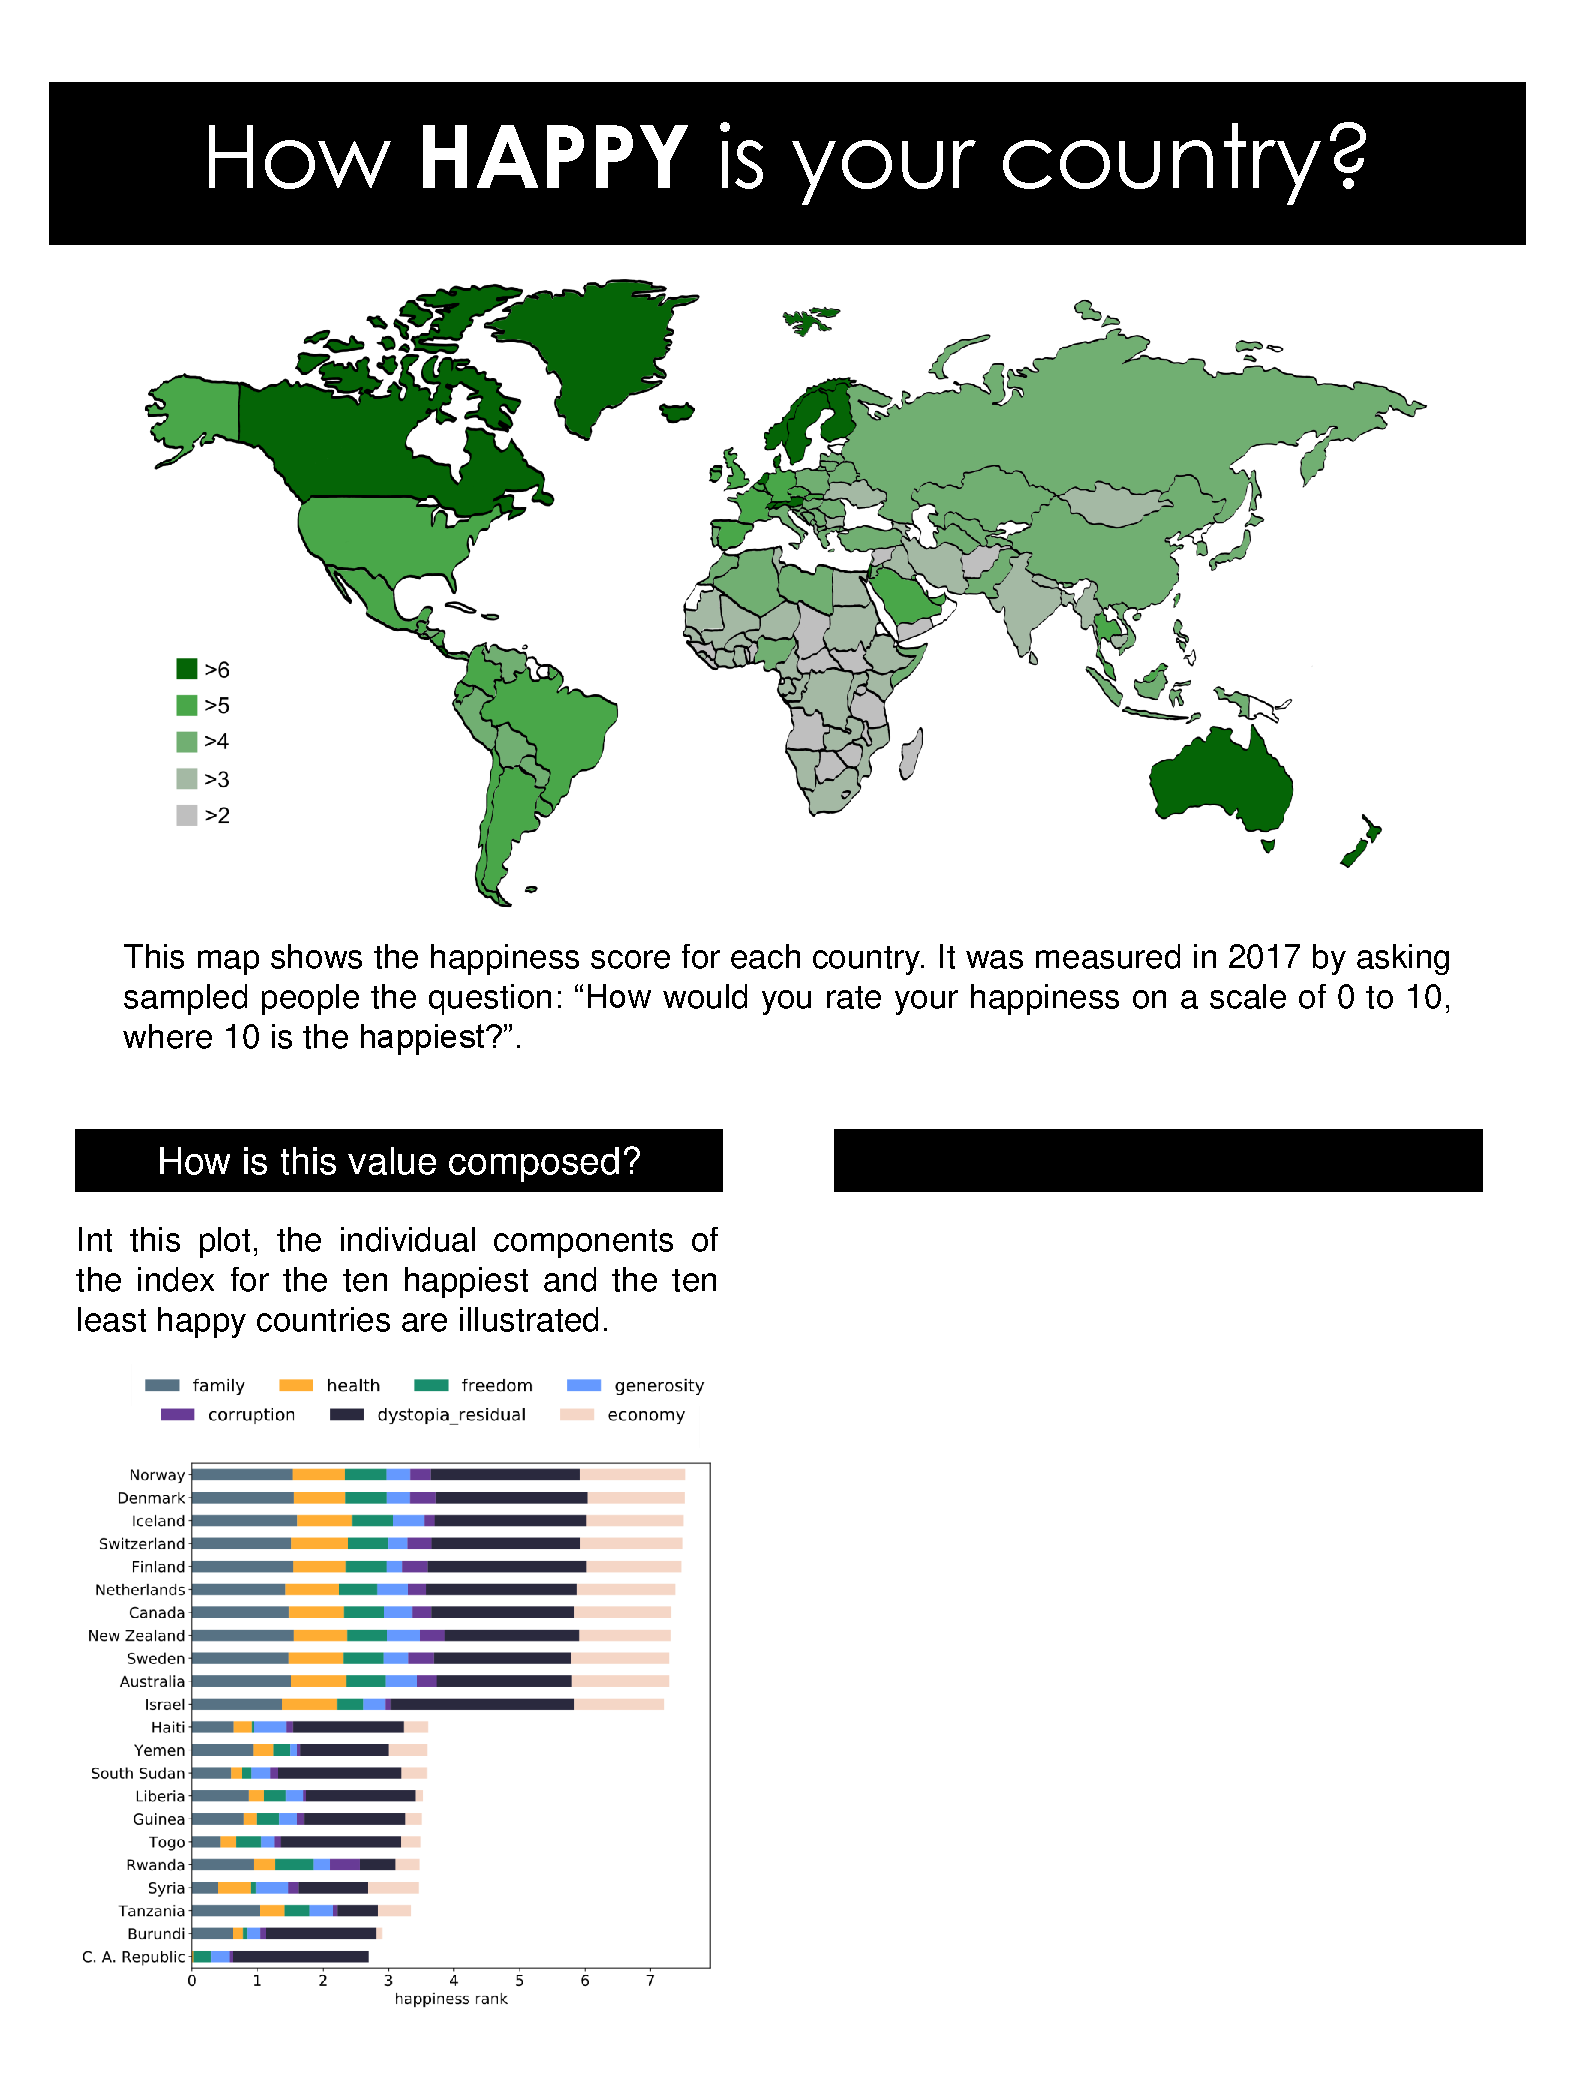
\includegraphics[width=0.98\linewidth]{HappyPoster.pdf}} \\

\section*{Task 1 - The happiness index by country}
\subsection*{(a) Visualizing the data}
%In either case, reflect and report in 3-10 sentences on the message of your poster/dashboard: if it is a storytelling assignment, what is the point of view you are conveying? if it is a data exploration assignment, what are potential conclusions an external viewer of your visualization might reach upon inspecting/reading your poster?
Our poster consists of three parts: first of all, there is a map at the top which shows the happiness score for each country on a map. 
This is supposed to give a quick overview on how the happiness is distributed across the world. 
Of course, this does not show any detail on the exact scores, therefore we created the more detailed visualisations at the bottom. 
The viewer could potentially see, that people in Africa seem to bee not as happy as in America or Europe.  
At the lower left corner, there is a bar chart which shows the ten happiest and least happy countries. 
The ranking can be easily seen, as well as the difference between each country. 
Besides that, it shows the composition, which is also interesting, because it is possible to dertermine whether one of the influencing factors is weaker or stronger in happy countries compared to sad countries. 
For example, a relation between the grey areas on the map above and the health component can be seen here. 
The viewer might conclude that for example worse health and less freedom might be corelated to the low happiness scores in many African countries. 
So, these two visualisations cover the happiness score and how it is composed in detail. 
The third visualisation at the bottom right corner covers a different topic. 
It shows that even if the freedom in this country is high, the internet access must be high as well to result in high happiness. 
Since scatter plots might not be as easy to understand as the map or bar chart, there is a bit more text description to help viewer understand what is illustrated here. \\ \linebreak
% Briefly report on weaknesses and strengths of your visualization, as well as potential improvements.
One strength of this visualisation is the map. 
It is easy to understand and interesting for all kinds of people, even those wo do not like to interpret charts. 
One disadvantage is, like mentioned above, that it is not very accurate or detailed. 
however we tried to adress the detail aspect with the lower plots. 
The advantage of the left plot is that it shows a lot of details in one bar, without being to overwhelming. 
People who are not interested in the exact components can still see the ranking and difference between the countries. 
It might be interesting to see more countries, but at the same time this would be overwhelming since 150 countries are a lot. 
In addition to showing the top and bottom 10 countries it might be interesting to see some countries in the middle. 
The right plot shows the least info. 
There are only 3 different variables. This was done to avoid visual clutter. 
It would have been possible to show much more information since the dataset contains a lot of useful data, but we decided to only illustrate interesting data as to not overwhelm the viewer. 
Additionally, it would have been possible to display the correlation between more than two columns like in the lower right plot, like for example in a scatter plot matrix, but we were not sure how easy people could understand this without spending to much time in front of the poster. 
The goal of our poster is therefore to give a quick overview with additional details. Showing more details would also be great if people are willing to spend more time to understand the poster. 


\subsection*{(b) Evaluation}
\subsubsection*{Methodology}
We evaluated our poster by having three people read it simultaneously. 
This way, they could instantly communicate their conclusions with each other, which in our opinion more closely resembles a situation in which a poster would be used than interviewing them one at a time.
Any questions they had regarding the data and its representation where answered by us and noted down.
Finally, we asked a few questions ourselves. These questions where:
\begin{enumerate}
\item[•]Did you understand the information in the poster? What was useful, what was not?
\item[•]What message does the poster convey? do you agree?
\end{enumerate}
\subsubsection*{Results}
As expected, the first part of the poster (the map) did not take long at all to be understood. 
Our participants initially took around five seconds to internalize it and did not have any questions about it. 
They did, however, talk among themselves avbout it, indicating it was still an interesting piece of information. 
The ease of understanding is likely due to this part's low information density and intuitivity.\\
For the second visualization, reading time, while still acceptable, appeared to be significantly slower (around 20-30 seconds). One comment we got was that the colors used for 'corruption' and 'dystopia residual' were too similar, making it hard to distinguish them. 
This could be fixed by either separating these two attributes or using different colors for them.
Another remark was that the meaning of 'dystopia residual' was not clear at all.
Here, a different label such as 'other' or 'unaccounted for', while not completely true to the original data, might be more useful in improving how easlily the visualization can be understood.\\
The third visualization was seen the most critical by our participants. 
The first point of contention was the color coding, i.e. it was not clear that the colors and associated numbers represent the position in the global ranking. 
To one of the participants, it was not immediately obvious that each dot represents a country at all.
another problem they had were the chosen attributes: since freedom and internet access seem to be related, it is not easy to make out whether it is internet access or freedom itself that makes people happy or if there is any causal relation at all.\\
The questions we asked afterwards revealed that while we did have to elaborate on some details (especially in vis.3), for the most part, our participants understood the poster and the narative it is trying to tell. 
Furthermore, they agreed with it's stance on internet access as an important factor of happiness.
However, this sentiment seemed to be informed less by the information given to them and more by previously held believes.
They were not convinced that internet access was a cause of happiness and suggested that instead other factors such as wealth might be a cause of higher happiness as well as higher internet access.


\end{document}
